\documentclass[solution, letterpaper]{cs121}

\usepackage{graphicx}

%% Please fill in your name and collaboration statement here.
%\newcommand{\studentName}{Renzo Lucioni and Daniel Broudy}
%\newcommand{\collaborationStatement}{I collaborated with...}
\newcommand{\solncolor}{red}
\begin{document}

\header{2}{April 4, 2013, at 11:40 AM}{}{}

%%%%%%%%%%%%%%%%%%%%%%%%%%%%%%%%%%%%%%%%%%%%%%%%%%%%
\section*{Analytical Approach}

\hspace{4mm} The conventional algorithm requires $n^3$ multiplications and $n^2(n-1)$ additions. Thus, the work required by the conventional algorithm, used when $n \leq n_0$, is $n^3 + n^2(n-1) = 2n^3 - n^2$. Strassens's algorithm requires 7 matrix products per recurrence, 10 additions and subtractions when deriving the $P_1, \ldots, P_7$, and 8 additions and subtractions when manipulating the $P_i$'s to find the matrix sums. The work required by Strassen's algorithm, used when $n > n_0$, can be represented by the recurrence $T(n) = 7T(\frac{n}{2}) + (10+8)\frac{n^2}{4} = 7T(\frac{n}{2}) + \frac{9}{2}n^2$, where $T(1) = 1$. Using Mathematica, we find that the solution to this recurrence with the given initial condition is $T(n) = 7^{(\log_2 n) + 1}-6 n^2$. This gives us the following function, which we wish to minimize over all $n$:
\[
    f(n)= 
\begin{cases}
    7^{(\log_2 n) + 1}-6 n^2, & \text{if } n > n_0 \\
    2n^3 - n^2, & \text{if } n \leq n_0\\
\end{cases}
\]

We can analytically determine the value of $n_0$ that optimizes the running time of the variant of Strassen's we are studying by setting equal both cases contained in $f$ and solving for $n$. Using Mathematica to solve the equation $7^{(\log_2 n) + 1}-6 n^2 = 2n^3 - n^2$, we see that both sides are equal when $n = 1$ and $n \approx 654.031$. The former value of $n$ is uninteresting, since we already know that the base case of Strassen's algorithm (i.e., when $n=1$) functions the same as the conventional method. Thus, we have analytically determined that $n_0 \approx 654.031$.

\section*{Experimental Approach}

\hspace{4mm}We first implemented both the conventional algorithm for matrix multiplication. We then implemented Strassen's algorithm for matrices where $n$ is a power of 2. We extended this implementation for more general values of $n$ by padding with 0's, as suggested in the hints section of the spec. We tied the two algorithms together by adding a conditional to our implementation of Strassen's to check if the current dimension was less than or equal to the cutoff value; if so, we switch to running our implementation of the conventional algorithm from within Strassen's algorithm. 

We tested for the optimal value of $n_0$ by running our modified version of Strassen's algorithm on matrices where $n=500$ and $n=1000$. In both of these matrices, every element was randomly selected to be 0, 1, or 2. The graphs below show our results. In each, the compute time is averaged over six runs.

\begin{center}
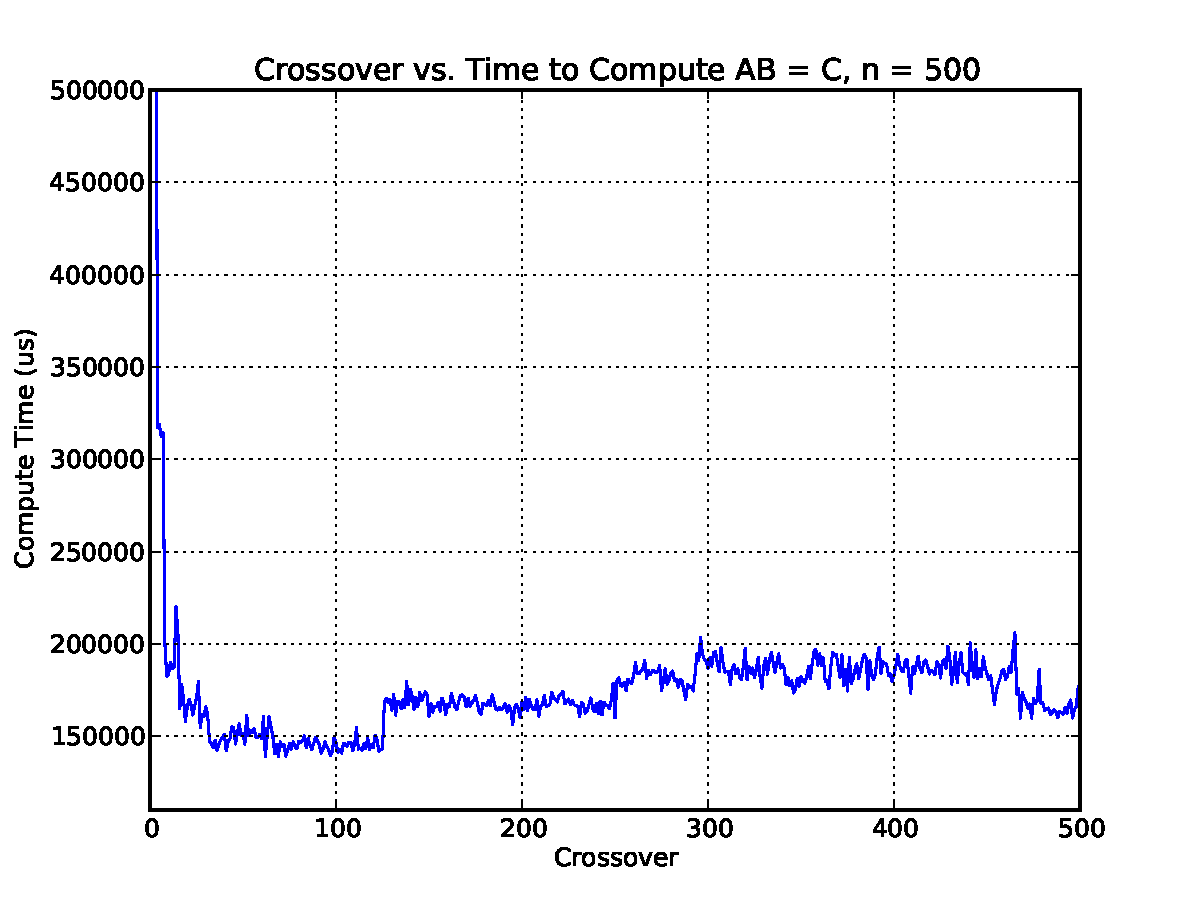
\includegraphics[scale=0.8]{crossover-v-compute-time-500.pdf}
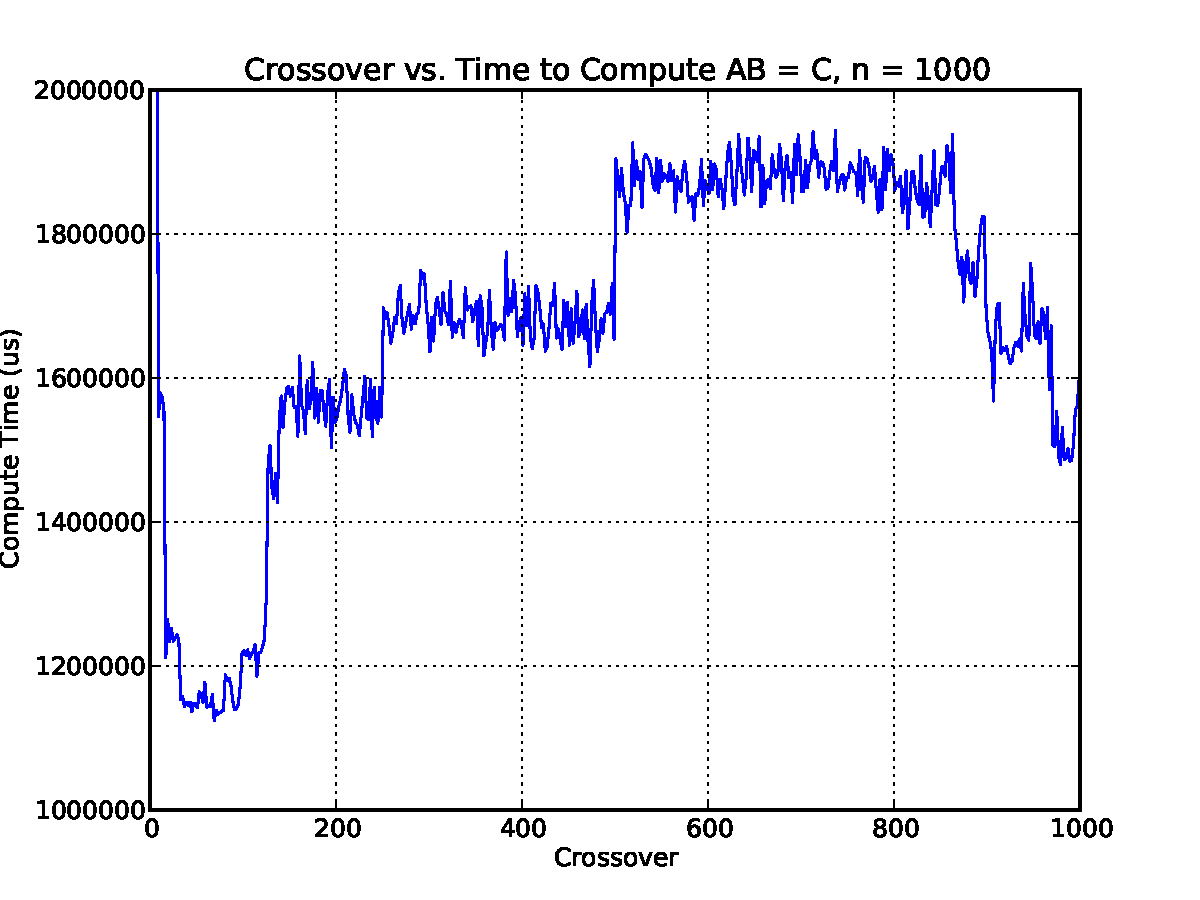
\includegraphics[scale=0.8]{crossover-v-compute-time-1000.pdf}
\end{center}

Notice the stepped pattern in the graph; each step occurs at a power at 2.

\section*{Discussion}

How low was our cross-over point? \\
What difficulties arose? \\
How did we speed things up? (took locality of reference into consideration when implementing conventional algorithm) \\
How large of an $n$ can we handle? \\
What types of matrices did we multiply (ints and floats), and does this choice matter? \\

\end{document}



